\section{Experimental Setup}
The parameter values used for the genetic programming algorithm have been mentioned throughout the preceding sections. Nevertheless, the most prominent parameters are as follows:

\begin{itemize}
    \item Population Size: 2048
    \item Crossover Rate: 0.9
    \item Mutation Rate: 0.05
    \item Reproduction Rate: 0.05
    \item Maximum Generations: 256
\end{itemize}

The data set used for training and testing can be found at \url{https://www.kaggle.com/sudalairajkumar/novel-corona-virus-2019-dataset}. Specifically, the data set comprising reported cases, deaths and recoveries between 22-01-2020 and 29-08-2020 was extracted from the aforementioned link. 

Furthermore, the data set was then split into a training set, used for the execution of the genetic algorithm, and an evaluation set, kept for cross-validation. Also, it is important to note that, due to the structure of the function and terminal sets, the first 30 days included in the data set were not directly used to evaluate fitness. The size and precise dates used for the split data set is shown in figure \ref{fig:data_sets}. This approach was heavily inspired by Hui \cite{hui2003using}.

\begin{figure}[H]
\centering
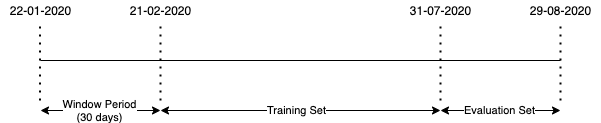
\includegraphics[width=\textwidth]{report/8_experimental_setup/data_sets.png}
\caption{Data Set Division}
\label{fig:data_sets}
\end{figure}

To test the algorithm a script was written which would run the algorithm on the data set with 10 different sets of seeds, writing the output of the program, it's execution time and the results of the algorithm to files which could be referenced later. The script is available in the github repository for this project (available at \url{https://github.com/marcus-bornman/cos_710_assignment_1}).

The machine used for development and testing purposes was a 2015 15-inch Macbook Pro with a 2.5 GHz Quad-Core Intel Core i7 processor, 16GB of memory and 500GB of storage. At the time of experimentation the machine had a battery cycle count of 684.